\chapter{Systeme}
\label{cha:systeme}

\section{Samsung Knox}

Als vorinstallierte Standardsoftware aktueller Samsung-Geräten findet man die App \textit{MyKnox}. Hiermit kann ein Benutzer mit einem einzelnen Tippen auf die Applikation zwischen gesichertem und normalem Modus wechseln. In diesem gesicherten Modus ist es durch eine Containerlösung möglich, Aktivitäten, geschäftlich oder privat, durch ein Sicherheitsverfahren zu schützen. Dieses Sicherheitsverfahren besteht bei der Knox-Plattform aus fünf Komponenten \cite{sam2017}:
\begin{enumerate}
\item Mehrschichtige Sicherheit
\item Root-of-Trust
\item Secure Boot und Trusted Boot
\item TrustZone®
\item SE for Android
\end{enumerate}


  Diese Knox-Plattform soll im Folgenden nach dem Kriterienkatalog betrachtet werden.
S
Samsung bietet je nach Sicherheitsanforderung verschiedene Softwarelösungen. Im Rahmen dieser Studienarbeit wird Knox Premium mit der Verbindung Knox Worksapace als Lösung genauer betrachtet.



\section{MobileIron}

\subsection {Allgemein} 
Das Unternehmen MobileIron ist ein US-amerikanisches Unternehmen mit Hauptsitz in Kalifornien welches im Jahr 2007 gegründet wurde. MobileIron hat sich von Anfang an auf die Verwaltung von mobilen Endgeräten im Enterprise Umfeld spezialisiert. Das Unternhemen wurde 2017 im siebten Jahr in folge als Leader im Magic Quadrant von der Gartner Inc. neben VMWare, IBM und BlackBerry für MDM/EMM Suites gekürt. Das Softwareentwicklungsunternehmen bietet in Ihrem Produktportfolio verschiedene Bring Your Own Device Pakete mit zahlreichen Funktionen an. 

\subsection {Paketmodelle}
MobileIron bietet die drei verschiedenen Bundles „EMM Silver“, „EMM Gold“ oder „EMM Platinum“ seiner Bring Your Own Device Lösung an.
Das Basispaket „EMM Silver“ beinhaltet die Komponenten „Core“ „Sentry „und „Apps@Work“. Das Paket „EMM Gold“ ist um die Module „Email+“, „Docs@Work“ und „Web@Work“ erweitert. Durch die Wahl des Platinum Pakets ergänzt sich dieses wiederum um „Help@Work“, „Tunnel“, „MobileIron Monitor“ und „ServiceConnect-Integration“.

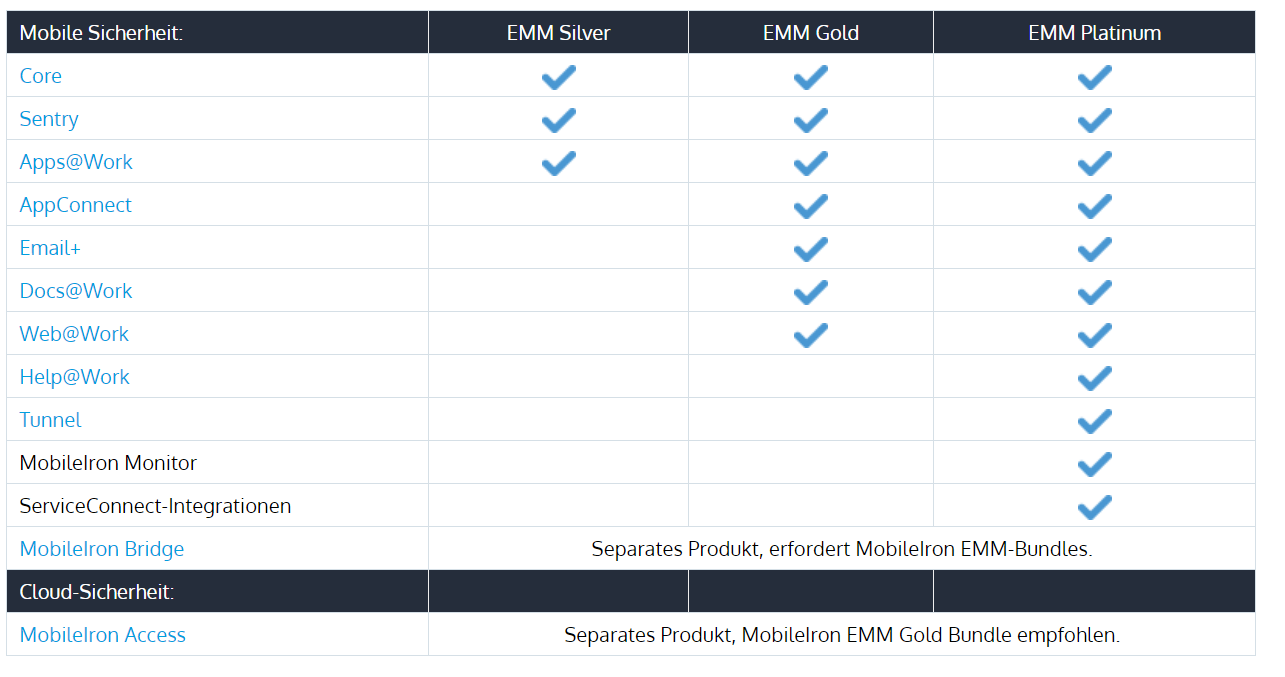
\includegraphics[width=0.95\textwidth]{Bilder/mi_1.png} 

\subsection {Abrechnungsmodell}

Je nach Tarifplänen bzw. Paketangeboten werden neben den genannten Grundfunktionen weitere Features unterstützt. Das Unternehmen selbst betreibt ein sehr flexibles Abrechnungsmodell, welches auf jegliche Bedürfnisse des Endkunden angepasst werden kann. Dabei kann beispielsweise zwischen einer Lizenzierung pro Benutzer (maximal 3 Endgeräte) oder einem Lizenzierungsmodell je nach Endgerät gewählt werden. Neben der Kaufoption von Lizenzen auf Lebenszeit wird auch ein Abonnement angeboten. 

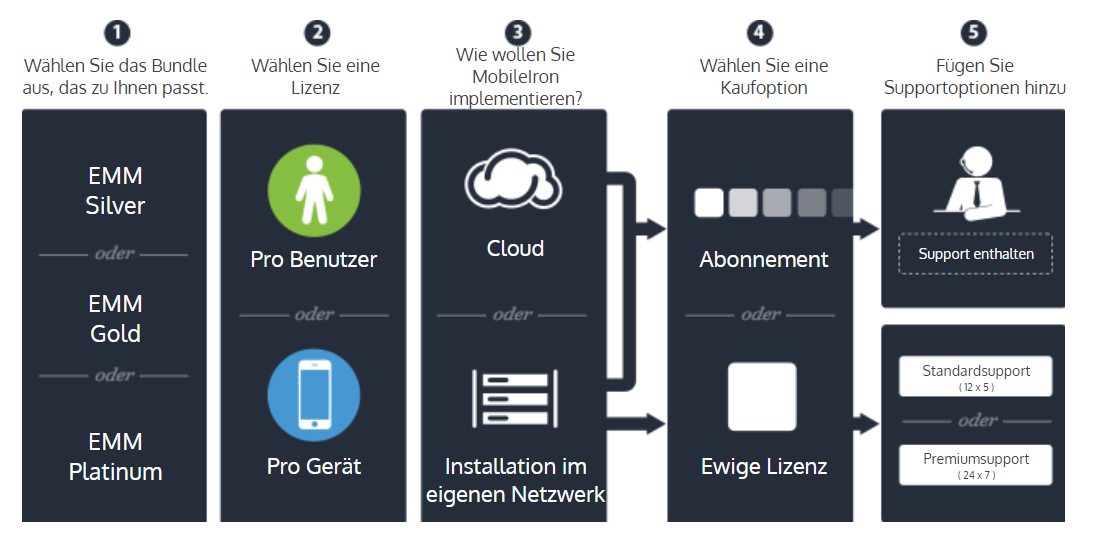
\includegraphics[width=0.95\textwidth]{Bilder/mi_2.png} 